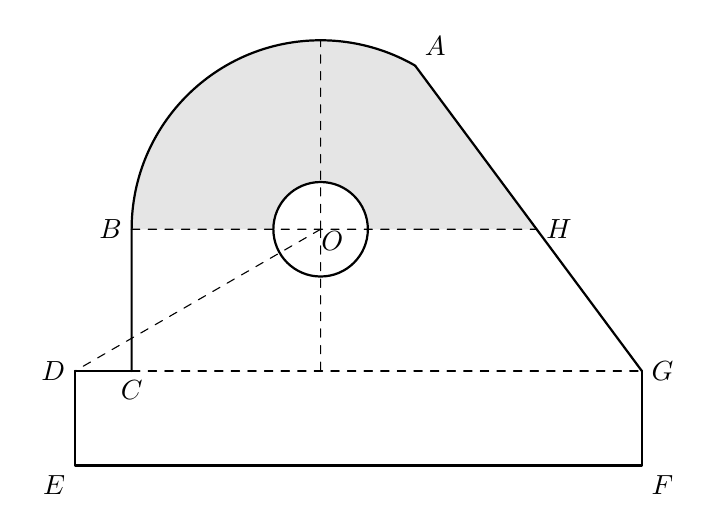
\begin{tikzpicture}[line cap=round,line join=round,scale=0.6]
\usetikzlibrary{calc,intersections}

\def\W{12}
\def\H{2}
\def\r{1}
\def\R{4}

\coordinate (E) at (0,0);
\coordinate (F) at (\W,0);
\coordinate (G) at (\W,\H);
\coordinate (D) at (0,\H);

\coordinate (O) at (5.2,5);
\coordinate (A) at ($(O)+(60:\R)$);
\coordinate (B) at ($(O)+(180:\R)$);
\path let \p1=(B) in coordinate (C) at (\x1,\H);

\path[name path=AG] (A) -- (G);
\path[name path=yfive] (-1,5) -- (\W+1,5);
\path[name intersections={of=AG and yfive, by=Hpt}];
\path let \p1=(O) in coordinate (Odown) at (\x1,\H);
\coordinate (Oup) at ($(O)+(0,\R)$);

\fill[gray!20,even odd rule]
  (B)
  arc[start angle=180,end angle=60,radius=\R] -- (G) -- (C) -- cycle
  (B) -- (C) -- (G) -- (Hpt) -- cycle;

\fill[white] (O) circle (\r);

\draw[thick] (D) -- (E) -- (F) -- (G);
\draw[thick] (D) -- (C);
\draw[dashed] (C) -- (G);
\draw[thick] (C) -- (B);
\draw[thick] (B) arc[start angle=180,end angle=60,radius=\R];
\draw[thick] (A) -- (G);
\draw[thick] (O) circle (\r);

\draw[dashed] (O) -- (Oup);
\draw[dashed] (O) -- (Odown);
\draw[dashed] (B) -- (Hpt);
\draw[dashed] (O) -- (D);

\node[left] at (B) {$B$};
\node[above right] at (A) {$A$};
\node[below] at (C) {$C$};
\node[left] at (D) {$D$};
\node[below left] at (E) {$E$};
\node[below right] at (F) {$F$};
\node[right] at (G) {$G$};
\node[right] at (Hpt) {$H$};
\node at ($(O)+(0.25,-0.25)$) {$O$};
\end{tikzpicture}